\documentclass[11pt,twoside,openany]{book}

\input macros


%\usepackage{tocloft}

%\renewcommand\cftchapafterpnum{\vskip-7pt}
%\renewcommand\cftsecafterpnum{\vskip5pt}



\begin{document}

\fontsize{13pt}{14.75pt}\selectfont %%linespread 1.04 (516) - finalized for second print

\frontmatter

\input src/000a-title
\newpage

\input src/copyright
\newpage

\pagenumbering{\select@language{kannada}}

\tableofcontents

%\setcounter{page}{1}
%\input src/000c-preface
%\newpage
%~\thispagestyle{empty}

%\newpage
%~\thispagestyle{empty}
%\vfill

%\begin{center}
%{\LARGE\bfseries ಕೊಲಂಬೊ ಇಂದ ಆಲ್ಮೋರಕೆ}
%\end{center}

%\vfill
%\newpage
~\thispagestyle{empty}
%\newpage


%\mainmatter

%\	rhead[]{{\fontsize{10}{12}\selectfont\leftmark\quad\arabictokannada{\thepage}}}
\newpage

~\thispagestyle{empty}

\begin{center}
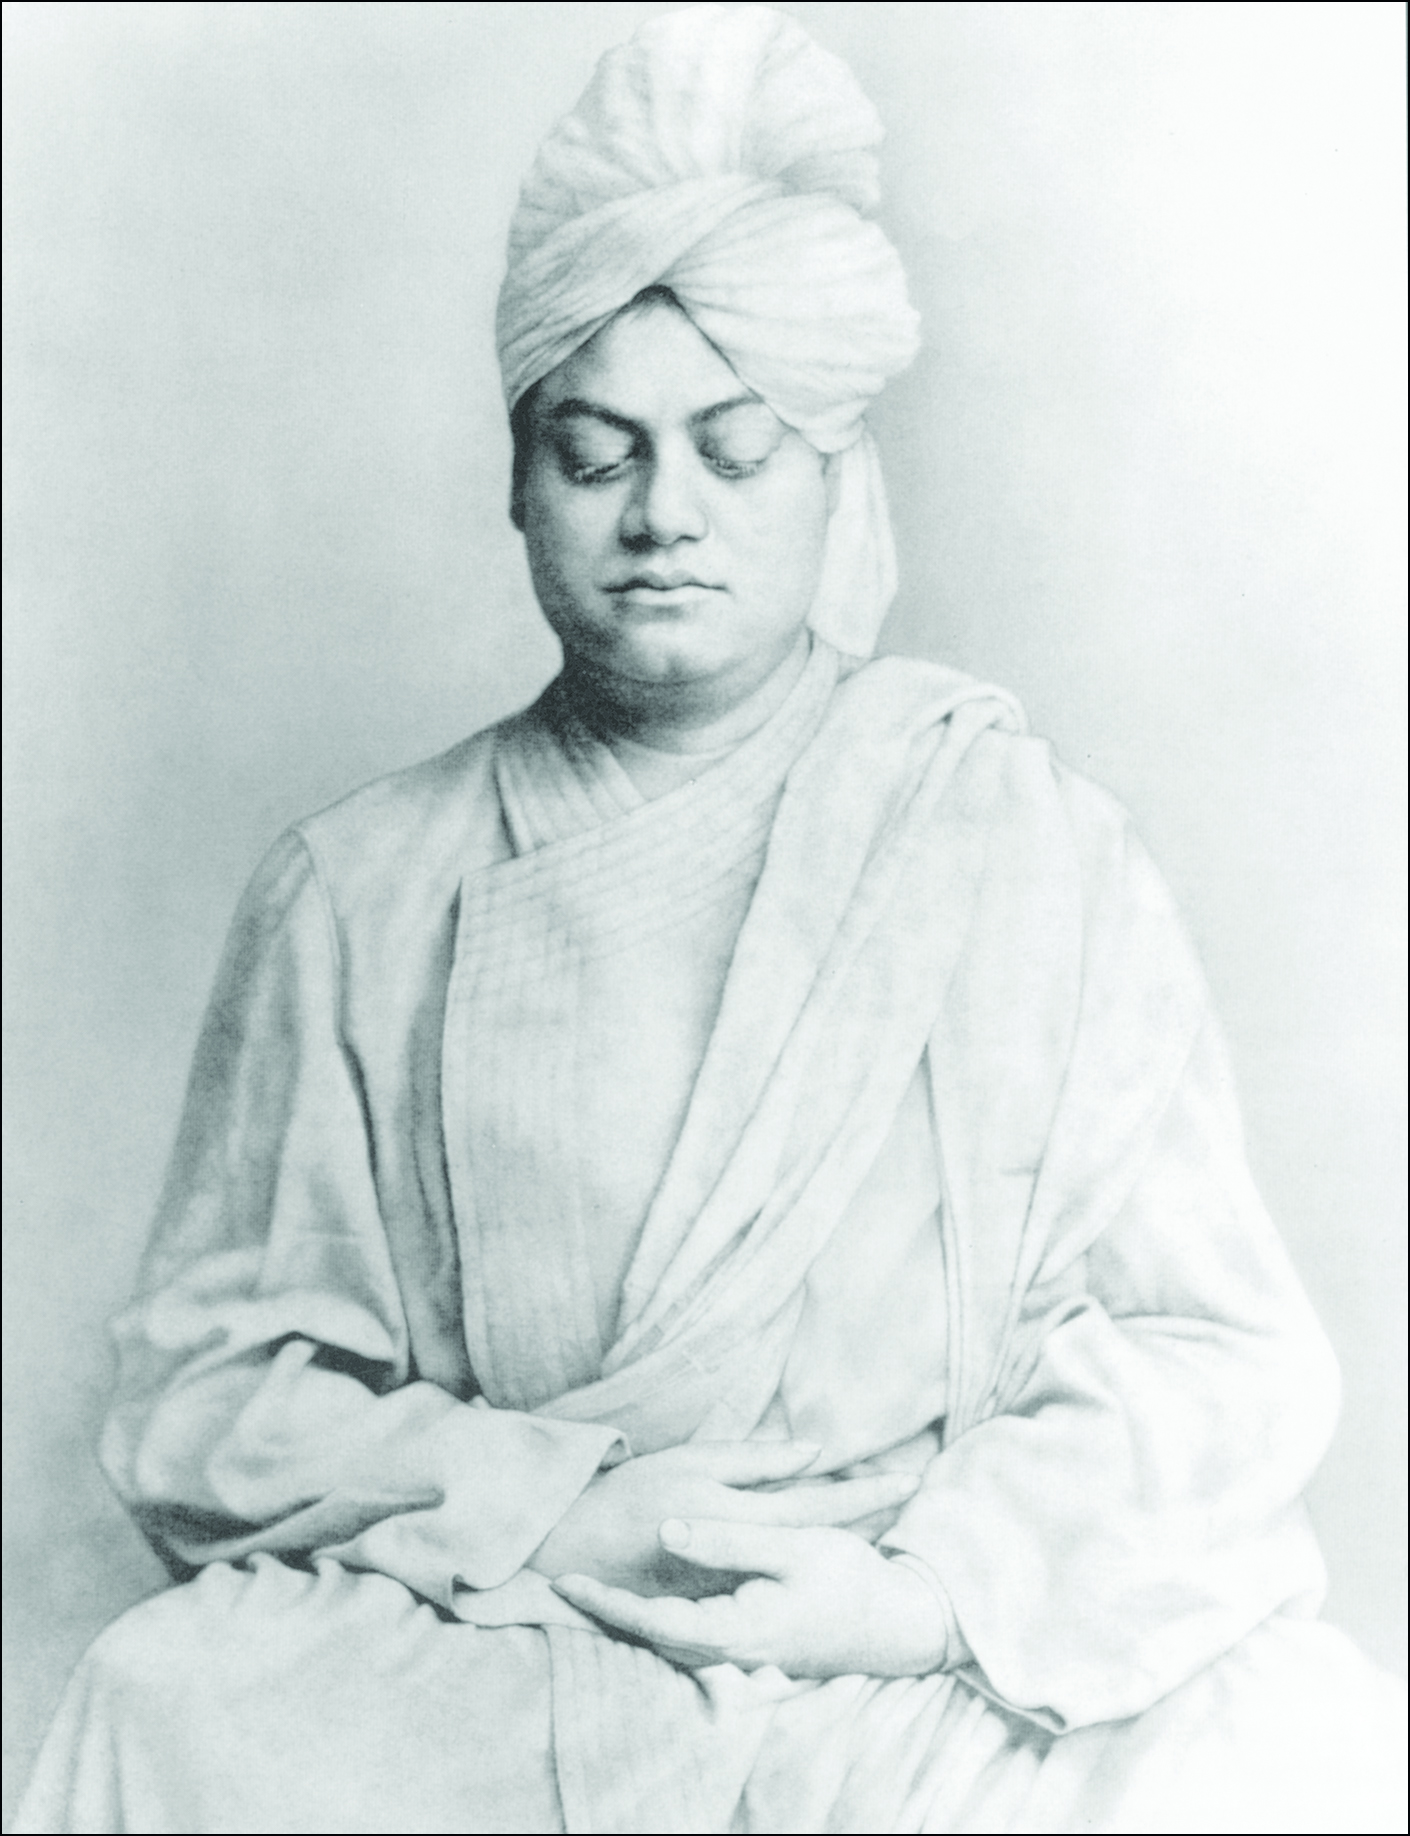
\includegraphics[scale=0.89]{images/SV21.jpg}
\end{center}

\newpage 

~\thispagestyle{empty}

\begin{center}
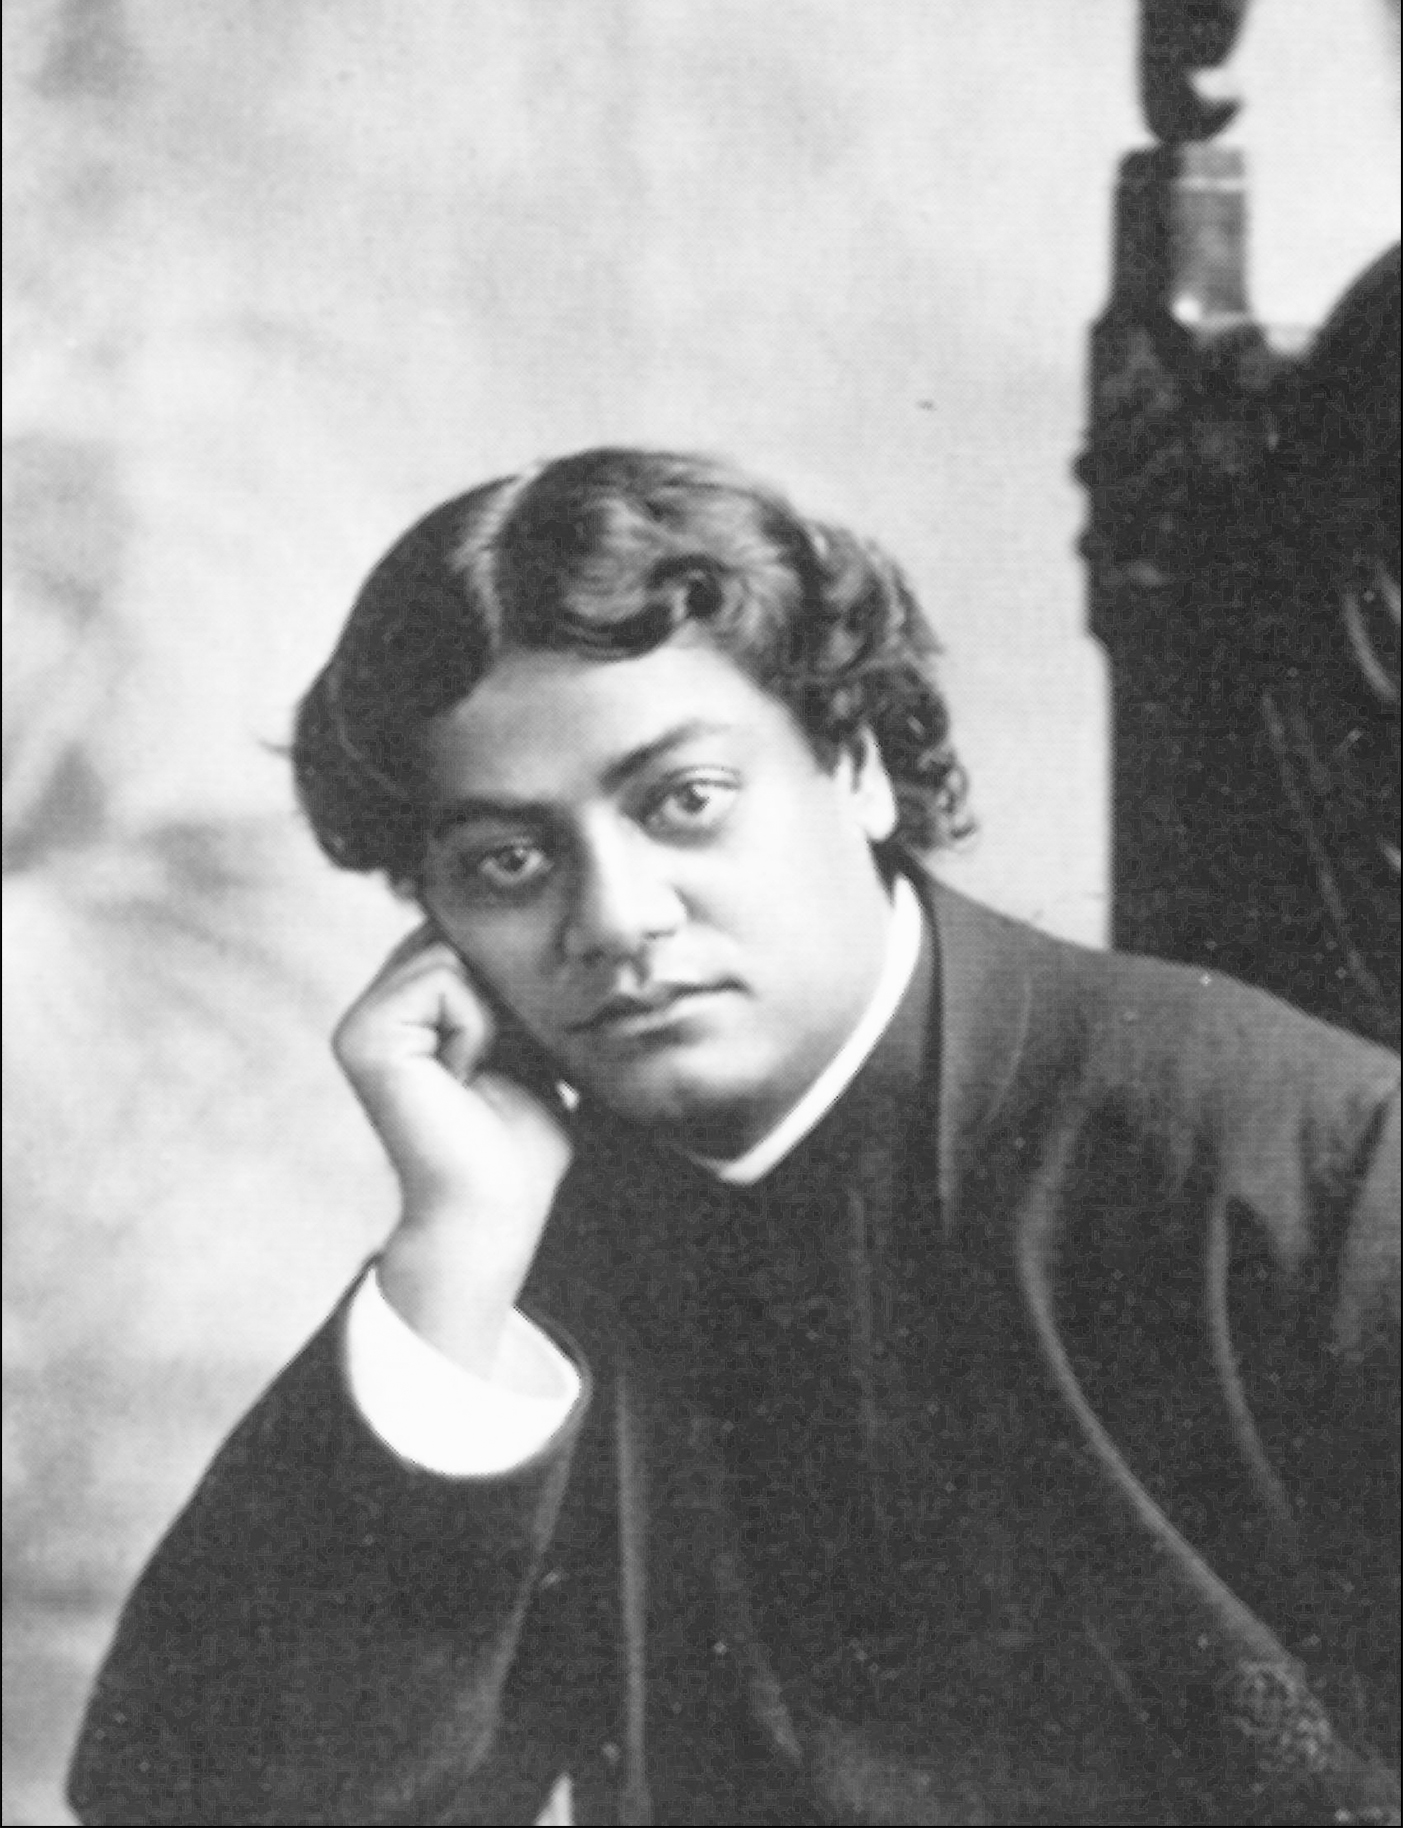
\includegraphics[scale=0.89]{images/SV22.jpg}
\end{center}

\mainmatter

\input src/001-chapter001.tex
\input src/002-chapter002.tex
\input src/003-chapter003.tex
\newpage

\vfill
\newpage
~\thispagestyle{empty}
\newpage


\makeatletter

\def\@makeschapterhead#1{%
  \vspace*{-60\p@}%
  {\parindent \z@ \raggedright
    \normalfont
    \interlinepenalty\@M
    \centering \Huge \bfseries ಶಬ್ದಸೂಚಿ\par\nobreak
    
    \vskip 2\p@
  }}

\renewcommand{\@idxitem}{\par\hangindent 20\p@}
\renewcommand*\subitem{\@idxitem \hspace*{10\p@}}
\renewcommand*\subsubitem{\@idxitem \hspace*{15\p@}}
\makeatother

\lhead[\small\arabictokannada{\thepage}\quad ಪದ ಸೂಚಿ]{}
\rhead[]{\small ಶಬ್ದಸೂಚಿ\quad\arabictokannada{\thepage}}
\label{index}
\printindex

\end{document}

